\chapter{Internal Implementation}
    \section{Overall}
        \begin{figure}[h]
            \centering
            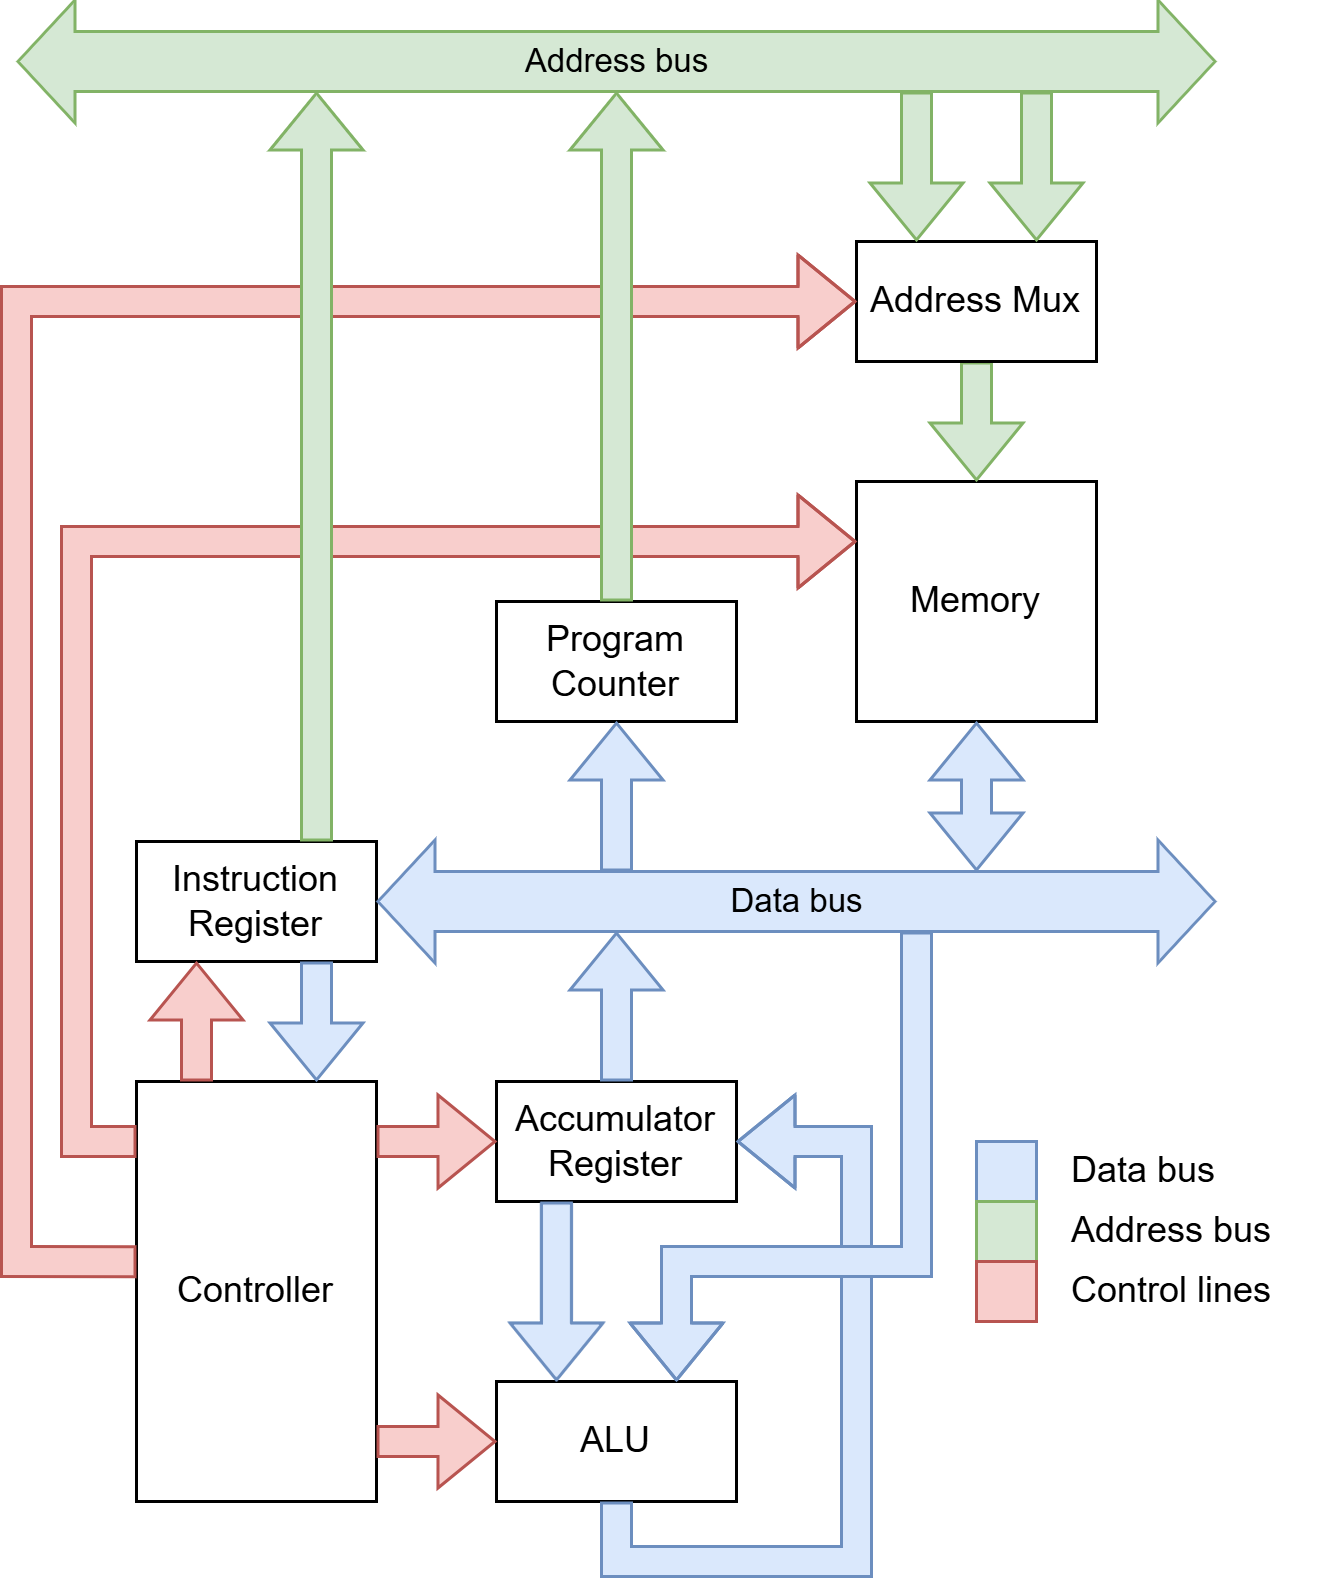
\includegraphics[width=0.6\textwidth]{graphics/RISC-CPU_simple.drawio.png}
            \caption{Sơ đối khối tổng quát của RISC-CPU}
        \end{figure}
        \newpage
        \begin{figure}[h]
            \centering
            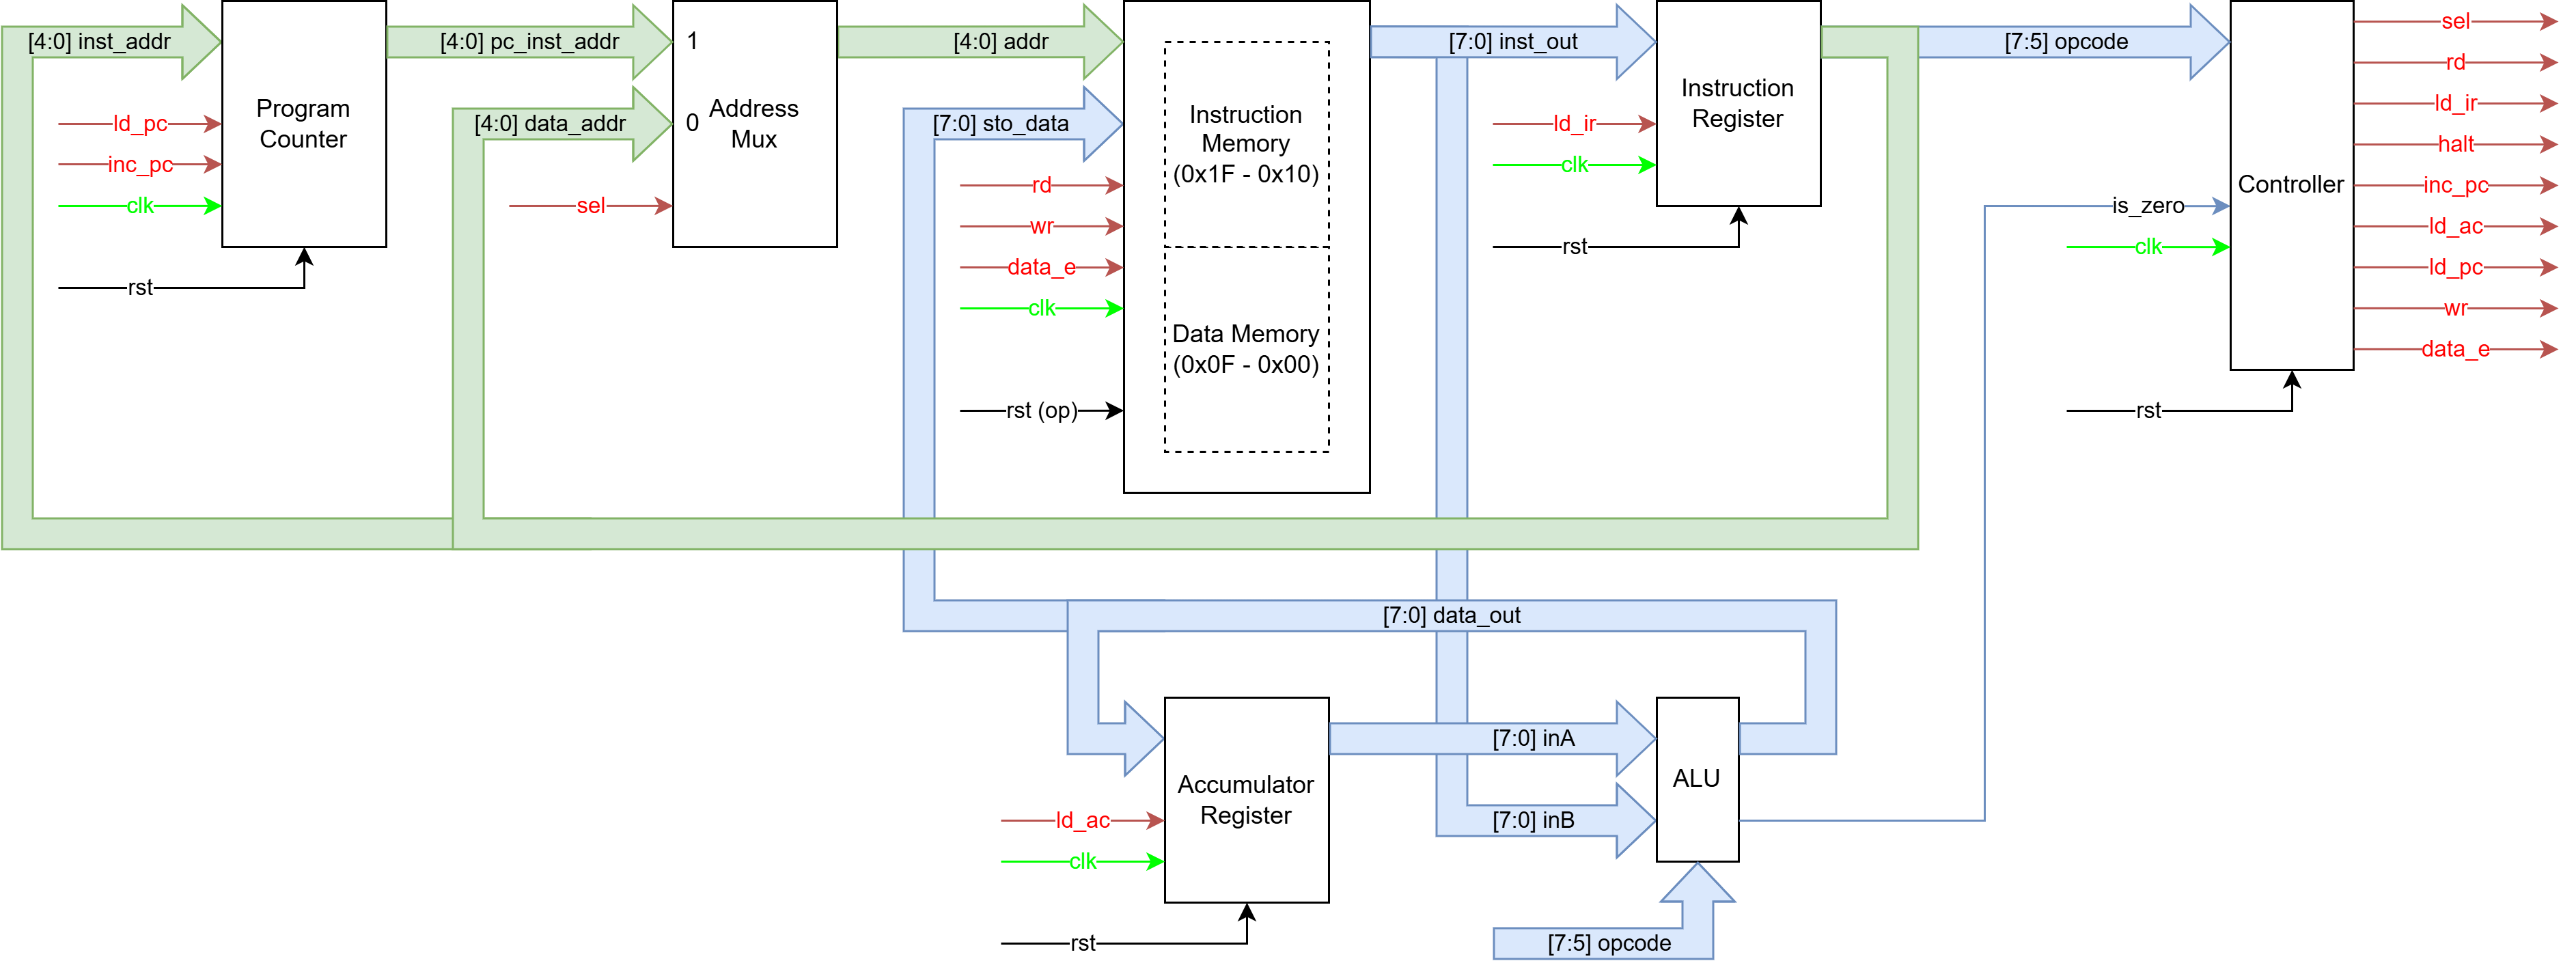
\includegraphics[width=0.8\textwidth]{graphics/RISC-CPU.drawio.png}
            \caption{Sơ đồ khối của RISC-CPU}
        \end{figure}


        \begin{longtable}{|p{0.2\textwidth}|p{0.15\textwidth}|p{0.15\textwidth}|p{0.4\textwidth}|}
            \hline
            \textbf{Tên tín hiệu} & \textbf{Khối phát} & \textbf{Khối nhận} & \textbf{Chức năng} \\
            \hline
            \endfirsthead
            
            \hline
            \textbf{Tên tín hiệu} & \textbf{Khối phát} & \textbf{Khối nhận} & \textbf{Chức năng} \\
            \hline
            \endhead
            
            \hline
            \endfoot
            
            \hline
            \caption{Mô tả tín hiệu của RISC-CPU}
            \endlastfoot
            
            \multicolumn{4}{|c|}{\textbf{Data bus}} \\\hline
            \texttt{inst\_out} & Instruction Memory & Instruction Register & Bus dữ liệu 8-bit tập lệnh. \\
            \hline
            \texttt{opcode} & Instruction Register & Controller, ALU & 3-bit opcode xác định loại lệnh đang thực hiện. \\
            \hline
            \texttt{inA} & Accumulator Register & ALU & Bus dữ liệu 8-bit đầu vào A cho ALU từ Accumulator Register. \\
            \hline
            \texttt{inB} & Data Memory & ALU & Bus dữ liệu 8-bit đầu vào B cho ALU từ Data Memory. \\
            \hline
            \texttt{data\_out} & ALU & Accumulator Register / Data Memory & Bus dữ liệu 8-bit kết quả phép toán từ ALU. \\
            \hline
            \texttt{sto\_data} & ALU & Data Memory & Bus dữ liệu 8-bit ghi vào Data Memory từ Accumulator Register. \\
            \hline
            \texttt{is\_zero} & ALU & Controller & Tín hiệu cho biết kết quả phép toán có bằng 0 hay không (dùng trong lệnh SKZ). \\
            \hline

            \multicolumn{4}{|c|}{\textbf{Address bus}} \\\hline
            \texttt{inst\_addr} & Instruction Register & Program Counter & Bus địa chỉ 5-bit dùng trong lệnh JMP. \\
            \hline
            \texttt{pc\_inst\_addr} & Program Counter & Address Mux & Bus địa chỉ 5-bit từ bộ đếm chương trình. \\
            \hline
            \texttt{data\_addr} & Instruction Register & Address Mux & Bus địa chỉ 5-bit để truy xuất dữ liệu từ Data Memory. \\
            \hline
            \texttt{addr} & Address Mux & Memory & Bus địa chỉ 5-bit được chọn để thực thi lệnh hoặc truy xuất dữ liệu từ Memory. \\
            \hline
            
            \multicolumn{4}{|c|}{\textbf{Control lines}} \\\hline
            \texttt{sel} & Controller & Address Mux & Chọn nguồn địa chỉ: địa chỉ lệnh hoặc địa chỉ dữ liệu. \\
            \hline
            \texttt{rd} & Controller & Memory & Kích hoạt chế độ đọc từ bộ nhớ. \\
            \hline
            \texttt{ld\_ir} & Controller & Instruction Register & Cho phép nạp dữ liệu mới vào Instruction Register. \\
            \hline
            \texttt{halt} & Controller & CPU System & Dừng hoạt động của CPU. \\
            \hline
            \texttt{inc\_pc} & Controller & Program Counter & Tăng địa chỉ Program Counter để nạp lệnh kế tiếp. \\
            \hline
            \texttt{ld\_ac} & Controller & Accumulator Register & Cho phép nạp dữ liệu mới vào Accumulator Register. \\
            \hline
            \texttt{ld\_pc} & Controller & Program Counter & Cho phép nạp địa chỉ mới vào Program Counter (dùng trong lệnh JMP). \\
            \hline
            \texttt{wr} & Controller & Memory & Kích hoạt chế độ ghi xuống bộ nhớ. \\
            \hline
            \texttt{data\_e} & Controller & Memory & Cho phép truyền dữ liệu trên bus. \\
            \hline
            \texttt{clk} & Clock source & CPU System & Đồng bộ hoạt động hệ thống theo xung clock. \\
            \hline
            \texttt{rst} & Reset source & CPU System & Đặt lại các khối về trạng thái khởi đầu. \\
            \hline
        \end{longtable}

    \section{State Machine}
        \begin{figure}[h]
            \centering
            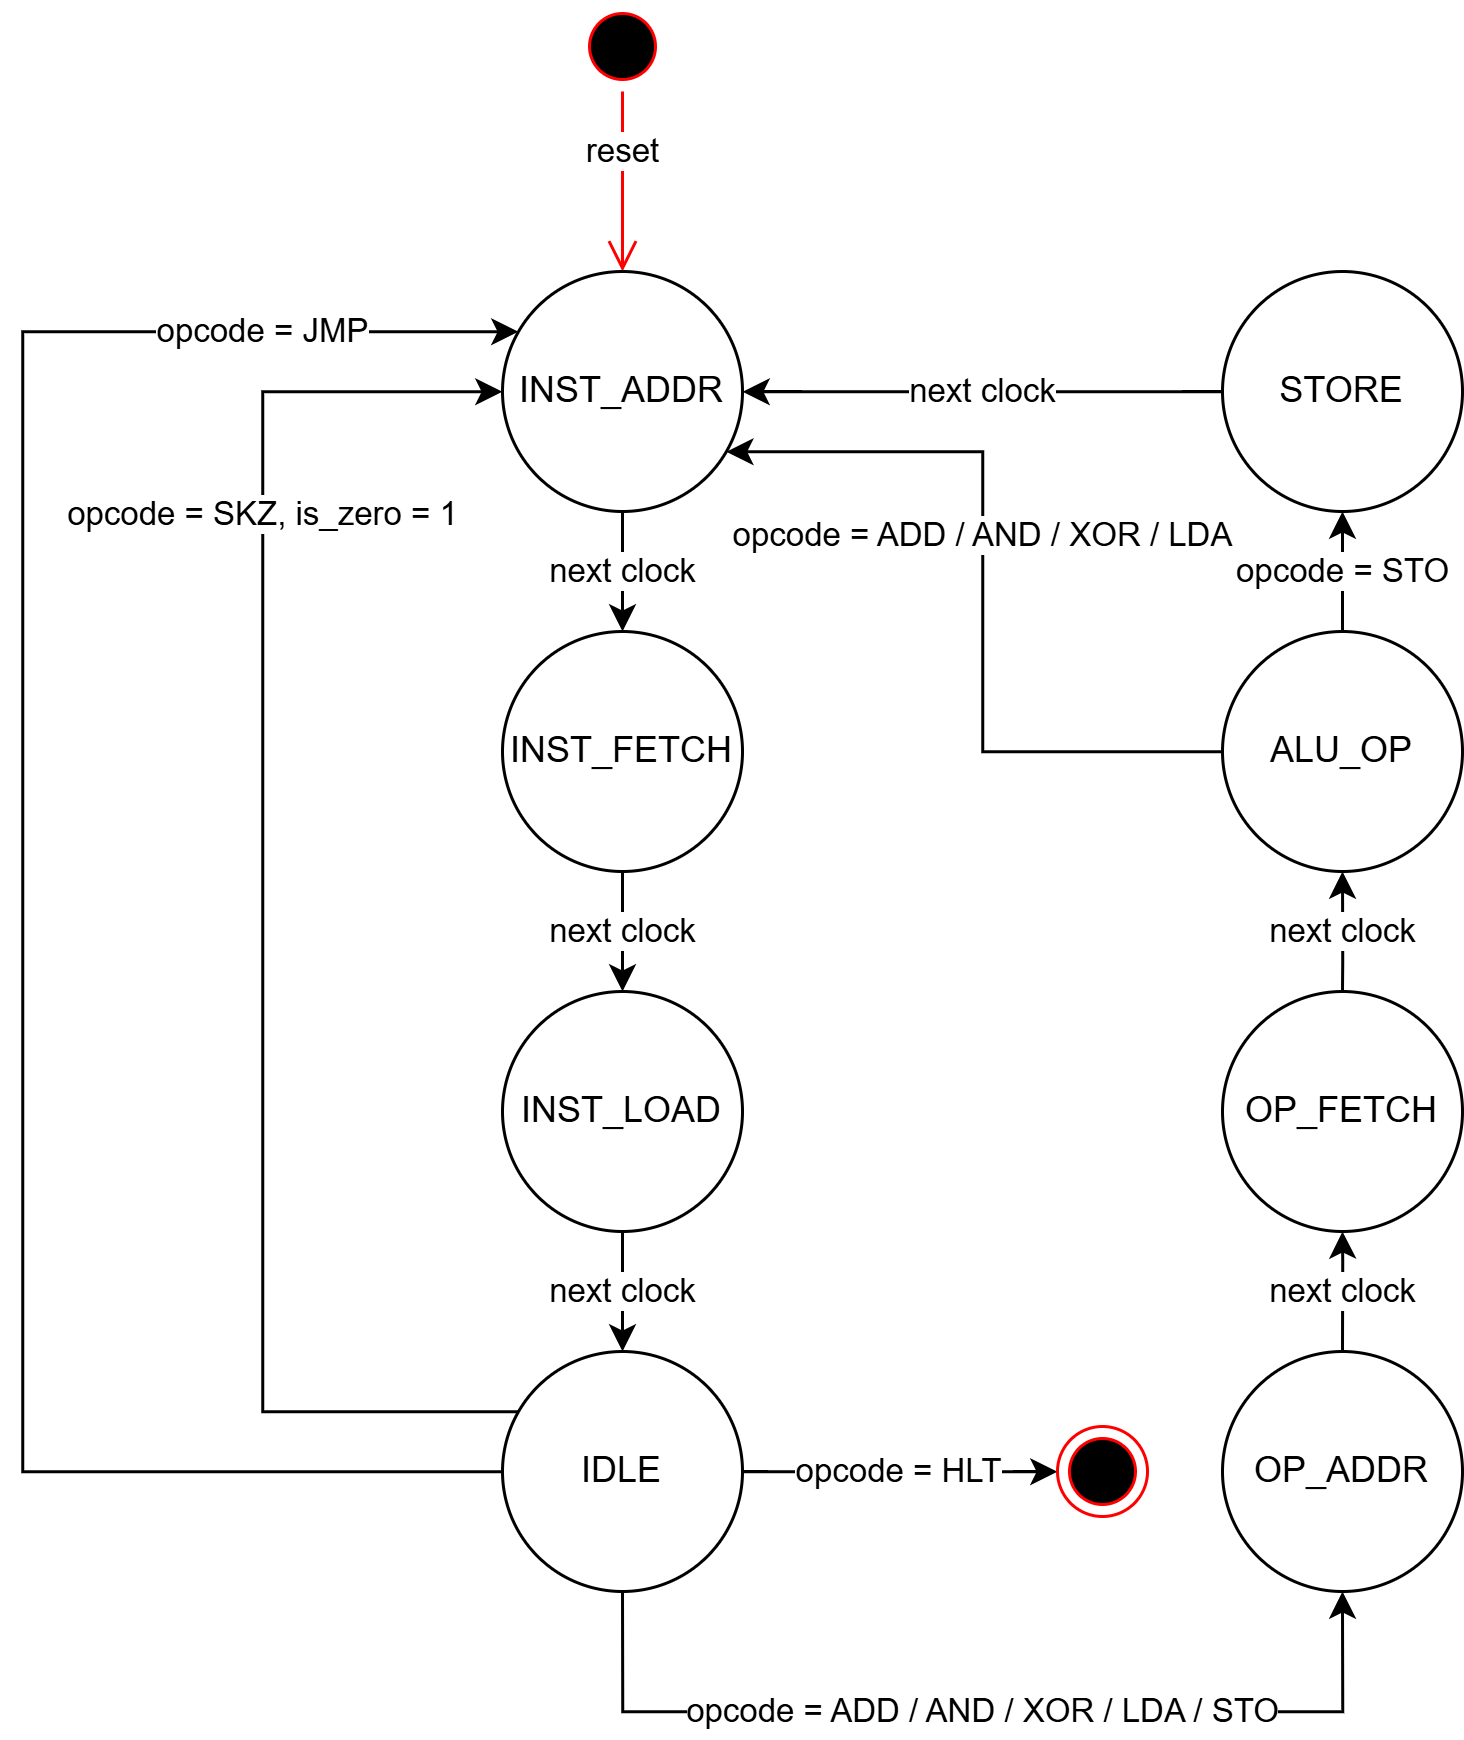
\includegraphics[width=0.8\textwidth]{graphics/RISC-CPU_FSM.drawio.png}
            \caption{Sơ đồ máy trạng thái của RISC-CPU}
        \end{figure}

        \begin{longtable}{|p{0.15\textwidth}|p{0.15\textwidth}|p{0.15\textwidth}|p{0.4\textwidth}|}
            \hline
            \textbf{Trạng thái} & \textbf{Điều kiện chuyển trạng thái} & \textbf{Trạng thái kế tiếp} & \textbf{Chức năng trạng thái} \\
            \hline
            \endfirsthead

            \hline
            \textbf{Trạng thái} & \textbf{Điều kiện chuyển trạng thái} & \textbf{Trạng thái kế tiếp} & \textbf{Chức năng trạng thái} \\
            \hline
            \endhead

            \hline
            \endfoot

            \hline
            \caption{Mô tả máy trạng thái của RISC-CPU}
            \endlastfoot

            \texttt{RESET} & Khi có tín hiệu \texttt{reset = 1} & \texttt{INST\_ADDR} & Đặt lại CPU, khởi động từ đầu chương trình. \\
            \hline
            \texttt{INST\_ADDR} & Sau 1 chu kỳ xung (\texttt{next clock}) & \texttt{INST\_FETCH} & Cung cấp địa chỉ lệnh từ PC để truy xuất lệnh từ bộ nhớ. \\
            \hline
            \texttt{INST\_FETCH} & \texttt{next clock} & \texttt{INST\_LOAD} & Đọc nội dung lệnh từ bộ nhớ. \\
            \hline
            \texttt{INST\_LOAD} & \texttt{next clock} & \texttt{IDLE} & Nạp nội dung lệnh vào Instruction Register. \\
            \hline
            \texttt{IDLE} & \texttt{opcode = HLT} & Dừng CPU & Kết thúc chương trình. \\
            \cline{2-4}
            & \texttt{opcode = SKZ} và \texttt{is\_zero = 1} & \texttt{INST\_ADDR} & Bỏ qua lệnh tiếp theo bằng cách tăng PC thêm 1 lần nữa. \\
            \cline{2-4}
            & \texttt{opcode = JMP} & \texttt{INST\_ADDR} & Nạp địa chỉ nhảy vào PC và tiếp tục thực thi từ địa chỉ mới. \\
            \cline{2-4}
            & \texttt{opcode = ADD / AND / XOR / LDA / STO} & \texttt{OP\_ADDR} & Bắt đầu xử lý các lệnh thao tác với bộ nhớ hoặc phép toán. \\
            \hline
            \texttt{OP\_ADDR} & \texttt{next clock} & \texttt{OP\_FETCH} & Cung cấp địa chỉ operand để truy xuất dữ liệu từ bộ nhớ. \\
            \hline
            \texttt{OP\_FETCH} & \texttt{next clock} & \texttt{ALU\_OP} & Đọc dữ liệu operand từ bộ nhớ. \\
            \hline
            \texttt{ALU\_OP} & \texttt{opcode = STO} & \texttt{STORE} & Ghi dữ liệu từ Accumulator xuống bộ nhớ. \\
            \cline{2-4}
            & \texttt{opcode = ADD / AND / XOR / LDA} & \texttt{INST\_ADDR} & Lưu kết quả phép toán vào Accumulator và quay lại vòng lặp lệnh. \\
            \hline
            \texttt{STORE} & \texttt{next clock} & \texttt{INST\_ADDR} & Ghi dữ liệu xuống bộ nhớ, sau đó trở về nạp lệnh mới. \\
            \hline
        \end{longtable}